\documentclass[a4paper]{article}

\usepackage{pdp}

%------------------------------------------------------------------------------
%	REPORT INFORMATION
%------------------------------------------------------------------------------

\title{Quoridor -- Python}
\subtitle{Rapport préliminaire}
\author{\begin{tabular}[t]{@{}l@{}}AIT-ISSAD MOHAMED SAID \\ BILAL AL FAYOUMI \\ GUILHEM CAUSSE \\ OMAR HARCHI \\ AMARA KOUSSAY\end{tabular}}

%------------------------------------------------------------------------------

\begin{document}

%------------------------------------------------------------------------------
%	TITLE PAGE
%------------------------------------------------------------------------------

\maketitle
\thispagestyle{empty}

%------------------------------------------------------------------------------
%	MAIN MATTER
%------------------------------------------------------------------------------

\section*{Introduction}

Quoridor is an abstract strategy board game designed by Mirko Marchesi and
first published in 1997 by the French company Gigamic. The game is played on a
square grid and is based on two simple actions: moving a pawn and placing
walls. Despite this apparent simplicity, the game exhibits a significant
strategic depth, as players must constantly balance progress toward their own
goal with the obstruction of their opponents.

The objective of this project is to design and implement a complete software
version of the game Quoridor, supporting two, three, or four players. The
program must strictly respect the official rules of the game and allow players
to interact through both a command-line interface and a graphical user
interface. In addition, the software must support configuration files,
internationalization, and robust error handling, in accordance with the
provided specifications.

This project goes beyond the development of a playable game. It aims to apply
fundamental software engineering principles, including modular architecture,
clear separation of concerns, automated testing, and comprehensive
documentation. Quoridor also represents an interesting case study from an
algorithmic perspective, as its gameplay can be naturally modeled using
graph-based representations and shortest-path algorithms, which are commonly
studied in computer science research.

\begin{figure}[H]
  \centering
  \begin{minipage}[t]{0.42\textwidth}
    \centering
    
\includegraphics[width=\textwidth]{resources/Logo_Gigamic_HD.jpg}
  \end{minipage}
  \hfill
  \begin{minipage}[t]{0.42\textwidth}
    \centering
    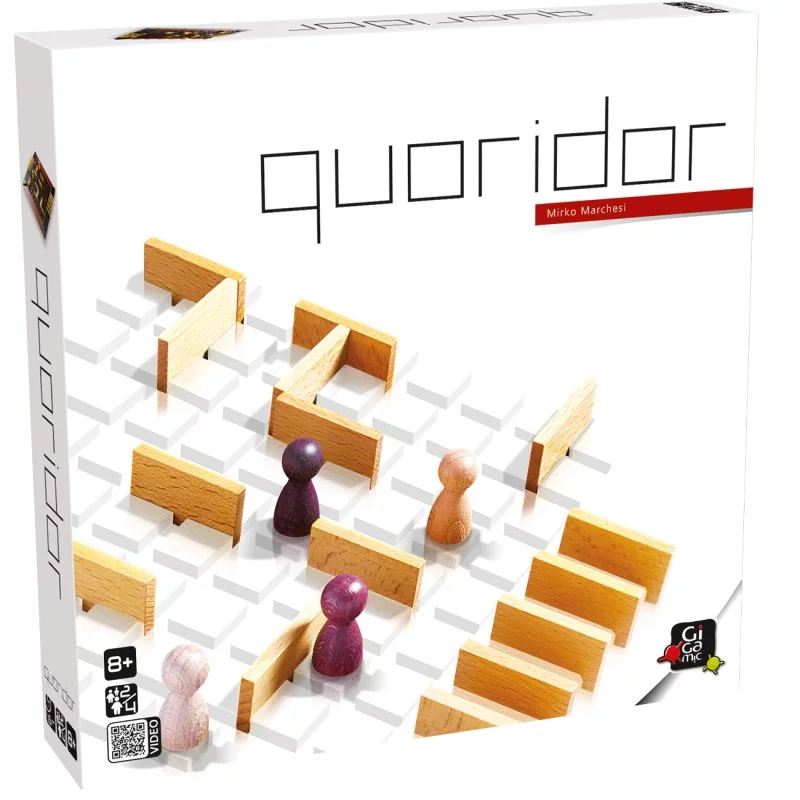
\includegraphics[width=\textwidth]{resources/boxquoridor.png}
  \end{minipage}
  \caption{Figure 1: Gigamic company (left) and Quoridor box (right)}
  \label{fig:gigamic-logo}
\end{figure}

\section{Historical Background and Existing Work}

Quoridor was invented by Mirko Marchesi in the mid-1990s and officially
released in 1997 by the French publisher Gigamic. Since its publication, the
game has gained international recognition for its elegant design and
educational value, receiving several prestigious awards such as the Mensa
Select Award in 1997 and the Games Magazine Game of the Year Award in 1998. Its
accessibility, combined with its strategic depth, has contributed to its
long-lasting popularity among both casual players and strategy game
enthusiasts.

Beyond its commercial success, Quoridor has attracted attention in academic
and technical contexts. The game's mechanics, which involve navigating a grid
while dynamically placing obstacles, make it a natural candidate for
algorithmic modeling. Several studies have explored Quoridor as a testbed for
artificial intelligence, pathfinding algorithms, and adversarial search
techniques.

In particular, previous academic work has shown that a Quoridor board can be
represented as a graph in which vertices correspond to board squares and edges
represent legal movements between adjacent squares. Wall placements
dynamically modify this graph by removing edges, while pawn jumps introduce
temporary alternative connections. Shortest-path algorithms such as
breadth-first search or Dijkstra's algorithm are commonly used to evaluate
positions, verify the legality of wall placements, and guide decision-making
in artificial intelligence agents.

Notable contributions include undergraduate and master-level research that
investigate heuristic evaluation functions, graph-based modeling, and search
strategies for Quoridor. These works highlight the computational complexity of
the game and demonstrate that, despite its simple rules, Quoridor poses
non-trivial challenges for both human players and automated systems. This
project builds upon these existing ideas while focusing primarily on the
design of a robust, extensible, and well-engineered software implementation.

\section{Première section}

Lorem ipsum dolor sit amet, consectetur adipiscing elit. Sed do eiusmod tempor
incididunt ut labore et dolore magna aliqua. Ut enim ad minim veniam, quis
nostrud exercitation ullamco laboris nisi ut aliquip ex ea commodo consequat.
Duis aute irure dolor in reprehenderit in voluptate velit esse cillum dolore eu
fugiat nulla pariatur. Excepteur sint occaecat cupidatat non proident, sunt in
culpa qui officia deserunt mollit anim id est laborum.

\section{Rules of the Game}

This section describes the official rules of Quoridor as implemented in this
project. The objective is to provide a precise and unambiguous description of
the game mechanics so that a complete game can be played without
interpretation issues.

\subsection{Board and Components}

Quoridor is played on a square board composed of a 9×9 grid, resulting in 81
playable squares. The squares are connected orthogonally, allowing movement in
the four cardinal directions. Between these squares, grooves allow walls to be
placed in order to block movement.

Each player controls a single pawn. In addition, a fixed number of walls is
available and distributed among the players at the beginning of the game.
Walls are barriers that block movement between adjacent squares and play a
central role in shaping possible paths across the board.

\subsection{Initial Setup}

At the beginning of the game, the board is empty except for the players'
pawns, which are placed at predefined starting positions.

In a two-player game, one pawn is placed at the center square of the bottom
row, while the second pawn is placed at the center square of the top row. Each
player's objective is to reach any square on the opposite side of the board.

In a four-player game, pawns are placed at the center of each side of the
board: one on the top, one on the bottom, one on the left, and one on the
right. Each player must reach the side opposite their starting position.

In the two-player configuration, each player receives ten walls. In the
four-player configuration, each player receives five walls in order to
maintain balance and avoid excessive blocking.

Players alternate turns, starting with one of the players chosen according to
the game configuration.

\begin{figure}[!ht]
  \centering
  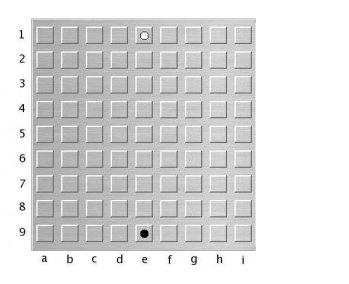
\includegraphics[width=.55\textwidth]{resources/quoridor-background.jpg.png}
  \caption{Quoridor board layout}\label{fig:quoridor-board}
\end{figure}

\subsection{Pawn Movement}

On their turn, a player may move their pawn to an adjacent square. Movement is
allowed only in the four orthogonal directions: forward, backward, left, or
right. Diagonal movement is not allowed under normal circumstances.

A pawn may only move to an adjacent square if there is no wall blocking the
path between the two squares. Pawns cannot move outside the boundaries of the
board, nor can they move onto a square already occupied by another pawn.

The goal of pawn movement is to progress toward the target edge of the board
while navigating around walls placed by the opponents.

\subsection{Jump Rules}
If a pawn is located directly adjacent to an opponent's pawn and no wall
separates them, the player may jump over the opponent's pawn. The jump moves
the pawn to the square immediately beyond the opponent's pawn in the same
direction.

If a direct jump is not possible because a wall blocks the square behind the
opponent's pawn or because the board edge is reached, the player may instead
move diagonally to one of the two adjacent squares to the left or right of the
opponent's pawn, provided no wall blocks that diagonal movement.

In four-player games, a pawn may only jump over a single pawn per move.
Multiple consecutive jumps over different pawns are not allowed.

These jump rules ensure that pawns cannot be completely blocked by the
presence of other pawns and that movement remains possible even in crowded
situations.

\begin{figure}[!ht]
  \centering
  \begin{minipage}[t]{0.32\textwidth}
    \centering
    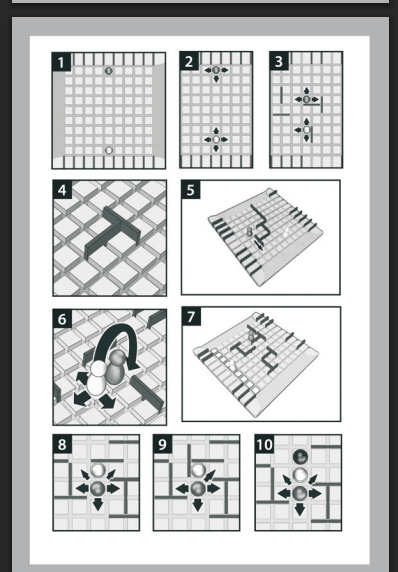
\includegraphics[width=\textwidth]{resources/deplacement.png}
    \caption{Pawn movement}\label{fig:pawn-move}
  \end{minipage}
  \hfill
  \begin{minipage}[t]{0.52\textwidth}
    \centering
    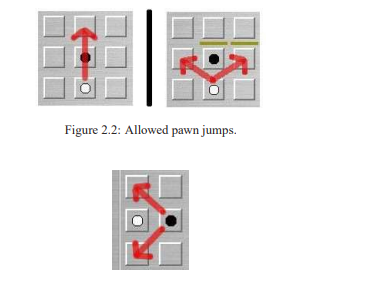
\includegraphics[width=\textwidth]{resources/allowed-jump.png}
    \caption{Allowed jump}\label{fig:allowed-jump}
  \end{minipage}
\end{figure}

\subsection{Wall Placement}

Instead of moving their pawn, a player may choose to place a wall, provided
they still have walls available. Walls are placed between squares and must be
oriented either horizontally or vertically. Each wall spans exactly two
adjacent square connections.

A wall placement must satisfy several constraints. Walls may not overlap or
cross existing walls, and they must fit entirely within the board's grooves.
Most importantly, a wall may not be placed if it completely blocks all
possible paths for any player to reach their target side.

To ensure this rule is respected, at least one valid path from each pawn's
current position to its goal edge must remain after the wall is placed. Pawn
positions do not block these paths, as pawns can always be jumped over under
the movement rules.

Once placed, walls are permanent and cannot be moved or removed for the
remainder of the game.

\subsection{Victory Condition}

The game ends immediately when a player moves their pawn onto any square of
their target edge. The first player to reach the opposite side of the board
wins the game.

In the standard rules of Quoridor, draws are rare and generally not expected
under normal play conditions, as players always have at least one legal move
available until a pawn reaches its goal.

Voici un exemple de code en Python :

{\large
  \begin{minted}[frame=single]{python}
def hello_world():
    print("Hello, World!")
hello_world()
  \end{minted}
}

Un exemple d'image flottante (Fig.~\ref{fig:example}).

\begin{figure}[!ht]
  \centering
  \frame{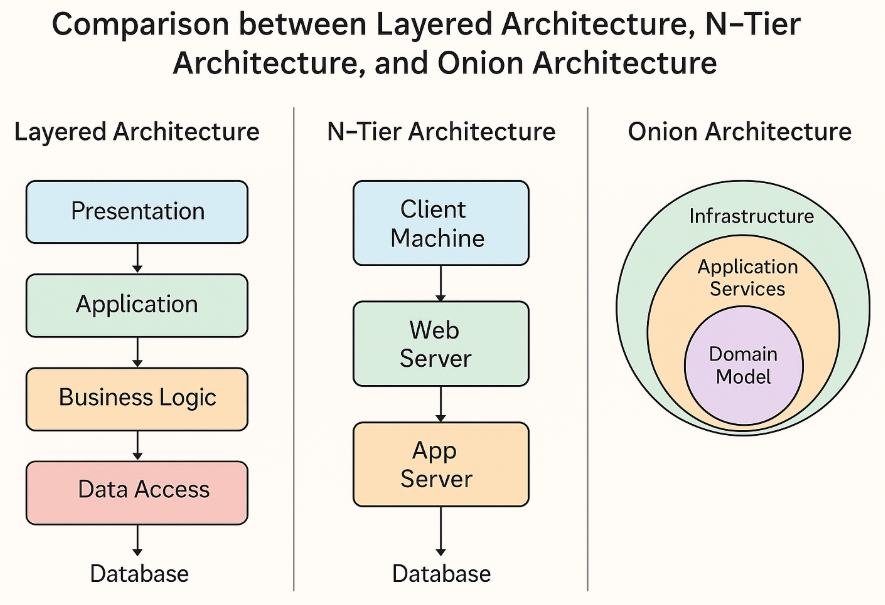
\includegraphics[width=.85\textwidth]{layered_architectures.png}}
  \caption{Une architecture en couches}\label{fig:example}
\end{figure}

\section*{Conclusion}

Suspendisse sit amet nisi placerat, vestibulum nisl vel, iaculis nunc.
Suspendisse quis libero vel ipsum gravida congue nec id arcu. Donec vel mi
viverra, commodo urna vitae, tincidunt lectus. Fusce pellentesque, lectus a
placerat vestibulum, magna lectus placerat nibh, vehicula pellentesque lacus
erat non nulla. Suspendisse maximus, turpis at suscipit egestas, libero massa
ultrices libero, at tincidunt velit eros a eros. Maecenas id tempor nunc.
Phasellus condimentum porttitor sapien in sagittis. Proin in metus diam. Mauris
in turpis sed ex viverra iaculis. Sed lobortis, tellus vitae congue blandit, leo
elit auctor libero, id tempor ante dolor quis quam. Donec eget ligula quam.
Maecenas porttitor massa vel felis elementum tristique.

%------------------------------------------------------------------------------
%	BIBLIOGRAPHY
%------------------------------------------------------------------------------

\nocite{*}
\bibliographystyle{plain}
\bibliography{bibliography}

%------------------------------------------------------------------------------
% BACK MATTER
%------------------------------------------------------------------------------
\appendix

\section{Section en annexe}

Lorem ipsum dolor sit amet, consectetur adipiscing elit. Sed do eiusmod tempor
incididunt ut labore et dolore magna aliqua. Ut enim ad minim veniam, quis
nostrud exercitation ullamco laboris nisi ut aliquip ex ea commodo consequat.
Duis aute irure dolor in reprehenderit in voluptate velit esse cillum dolore eu
fugiat nulla pariatur. Excepteur sint occaecat cupidatat non proident, sunt in
culpa qui officia deserunt mollit anim id est laborum.

\end{document}
